\documentclass[12pt]{article}
\usepackage[margin=.75in]{geometry}
\usepackage{textcomp}
\usepackage{float, graphicx, color, soul}
\usepackage{amsmath}
\usepackage{listings}
\lstset{
basicstyle=\ttfamily,
frame=single,
numbers=left
}
\title{CS185C: \\ 
Final Project \\
Malware Classification}

\author{Jordan Conragan,  Brett Dispoto}

\begin{document}
\maketitle
\tableofcontents
\newpage

\part{Preprocessing}
\section{Preprocessing the Dataset}
Most of the machine learning techniques used in this report use variants of the same preprocessing steps. Here are the preprocessing steps taken for the methods described in this report. Preprocessing was done using both python and bash scripts. The relevant files can be found in the \texttt{preprocessingScipts} directory of our submission.
  \begin{enumerate}
  \item Download the dataset (\texttt{malicia} | provided by Fabio Di'Troia).
    \item Split the dataset into directories based upon their family label. (Already completed by the dataset provider.)
    \item For each malware family, the following steps were then taken:
      \begin{enumerate}
        \item Read through all of the files, count the occurrence of each unique opcode across all files.
        \item Take the $n$ (turning parameter) most common Opcodes, and convert them to an ASCII symbol for observation symbols for our HMMs. The Opcodes which are not within the $n$ most common will be converted to an "other" symbol. This will reduce noise in our model.
        \item Once each opcode is assigned a symbol, we again read through the files and convert the opcodes to symbols.

        \begin{enumerate}
          \item If bagging is being used, make copies of \textbf{each} converted malware file, which will later be split up accordingly during training.
          \item Otherwise, if boosting or stacking is being used, we can simply dump the converted opcodes (symbols) for the entire family into one huge file. This file will be our observation sequence.
        \end{enumerate}
      \end{enumerate}
  \end{enumerate}
\newpage

\part{Experiments}
\section{K-Nearest Neighbors}
K-Nearest Neighbors (KNN) was one of the first algorithms implemented in this work. KNN makes a wise first choise because it allows us to examine the dataset, potentially for intuitive solutions to building a model.

KNN was implemented following according to the following features of our samples:
  \begin{enumerate}
    \item Entropy of opcode sequence, and
    \item Number of distinct opcodes
  \end{enumerate}
  KNN is performed using the files \texttt{KNN.py} and \texttt{knnPreprocesor.py}. The procedures and results are described in the sections below. \textit{sklearn} was used as a KNN library for python.

\subsection{KNN Procedure}
  Procedures for running the KNN algorithm on the dataset is as follows:

  \begin{enumerate}
    \item Preprocess the dataset. This includes:
        \begin{enumerate}
          \item Convert all opcodes to symbols,
          \item Count the number of distinct symbols in each sample,
          \item Compute the entropy $H(X)$ of the sequence of opcodes. This is given by Shannon's Entropy:
          \begin{equation}
            H(x) = E[I_X] 
          \end{equation}
        \item Write the above information in a file for each sample.
        \end{enumerate}
      \item Use 90\% of the dataset as our "training" samples (there really is no training in KNN).
      \item Test KNN using 10\% of the dataset.
      \item Repeat steps 2 and 3 for different values of $K$, ranging from $2$ to $10$. Keep the best result.
  \end{enumerate}
  \subsection{KNN Results}
  Below are the results of the above procedure:

          \begin{figure}[H]
          \centering
          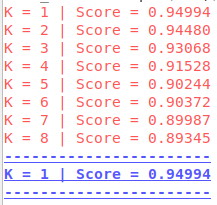
\includegraphics[width=0.3\textwidth]{knn.png}
          \caption{Finding the best value for $k$.}
          \end{figure}
 
  As can be seen above, the best achived accuracy using KNN is where $K=1$.
  
          \begin{figure}[H]
          \centering
          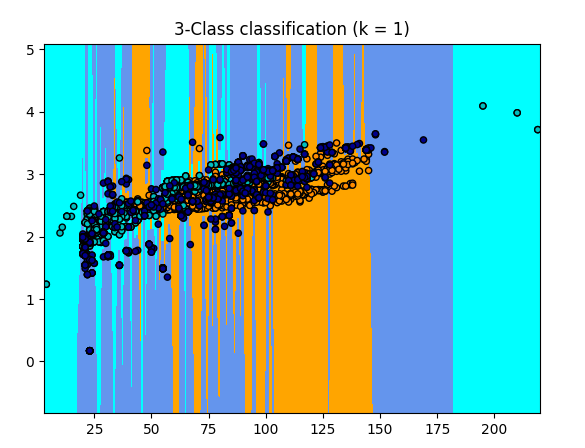
\includegraphics[width=0.55\textwidth]{k1.png}
          \caption{Family Clusters when $K=1$}
          \end{figure}
 
  When we plot the clusters on a graph, we can see that when $K = 1$, we can see that we're overfitting on the training set:


  Therefore, if this model were used in software production, we would probably choose a larger $K$ such as $K=3$ as to reduce overfitting. Below are the clusters when $K=3$:

          \begin{figure}[H]
          \centering
          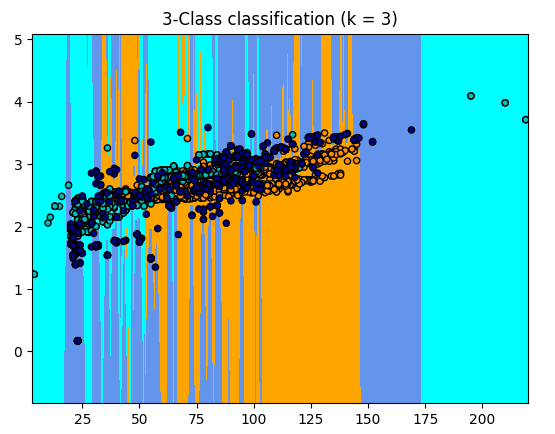
\includegraphics[width=0.5\textwidth]{k3.png}
          \caption{Initial results from Bagging.}
          \end{figure}

\section{Primitive SVM}
  \subsection{SVM Procedure}
  \subsection{SVM Results}

\section{HMM Bagging}
  Bagging is performed using the files \texttt{Bagging.java} and \texttt{HiddenMarkovModel.java}. The procedures and results are described in the sections below.
\subsection{Bagging Procedure}
  The following steps were performed in order to use bagging as an ensemble method:
  \begin{enumerate}
    \item Split assembly instructions into their appropriate family, and translate the instructions to HMM symbols,
    \item Within these family folders, use a shell script (included, \texttt{makeTesting.sh}) in order to split 10 percent of the samples into a test set.
    \item Train $x$ HMMs on each family,
    \item Once each HMM for a given family is trained, score the observation sequence which just used to train the model.
    \item Write down this score. 
    \item Once all HMMs of a given family are trained, use whichever ensembler aggregate function to take all the generated scores and aggregate them into one score. 
    \item Once training is complete for all families, for each family we now have this "aggregate score" written down in a log in the directory where the training samples are located.
    \item Finally, to test all of these trained HMMs, we go into all of the test sets, score the test sample using the \textbf{each of the three "ensemblers"} (each made up of $x$ HMMs.). Once we have the score from each ensembler, we can then go back to the logs where the original score was written down for the training samples. 
    \item Now, our sample has one score for each ensembler, denoted as $S_{1..\text{\texttt{num\_ensembler}}}(x_{\text{test}})$
    \item We classify this sample as whichever has the minimum of $abs(S_{\text{\textit{family}}}(x_{\text{test}}) - \text{\textit{score}}_\text{family} )$, that is, we classify as whichever family's "original score" score is closest to the score for the sample given by \textit{that family's} "ensembled" HMMs. In other words, we're just doing the KNN algorithm, where $k = 1$
  \end{enumerate}

\subsection{HMM Bagging Results}
  \subsubsection{Bagging Results}
  The best found bagging results are given in the below table:
  \begin{table}[H]
    \centering
  \begin{tabular}{|l|l|l|}
    \hline \textbf{Key} & \textbf{Value} \\\hline \hline
    Ensembler Aggregate Function & \textsc{MAX}  \\ \hline
    HMM's per ensembler & 10 \\ \hline
    N (HMM parameter -- \# states) & 2 \\ \hline
    Random initialization seed (HMM) & 0 \\ \hline
    Test set size  & 10\% of training set \\ \hline
  \hl{Test Accuracy} & \hl{0.9974326059050064}  \\ \hline
  \end{tabular}
  \end{table}
  As is shown in the table above, the first bagging experiments went well on the surface. Screenshots of the information described here can be found in figure [\ref{bagging1}] in the appendix.

  \paragraph{On the Result:}
  \begin{enumerate}
    \item Whenever a sample was scored \textbf{using an HMM which was NOT trained on the family which the sample belongs to, the score is returned as NaN.} This makes for very good accuracy; however, this behaver cannot be mathematically or otherwise justified.
      \begin{itemize}
        \item For example, if a \texttt{winwebsec} sample was scored using an HMM which was trained on samples form the \texttt{zbot} family, then all the \texttt{zbot} HMMs will give \texttt{winwebsec} samples a score of NaN. \textit{This was somewhat unexpected, because our HidddenMarkovModel implementation takes special caution (using logrythims) to avoid underflow. Further, we know our HMM is valid because of extensive testing using Mark Stamp's paper "A Revealing Introduction to Hidden Markov Models"}. Our intuition tells us that this is okay, because the samples are still being given a valid score when the correct family's HMM's is used.
        \item To attempt to remedy this, we tried changing training methodology:
          \begin{enumerate}
            \item \textbf{Increase number of HMMs} | Currently, durring training, when an HMM is trained on an observation sequence, that observation sequence is much, much larger than the actual samples which are being scored. To remedy this, we can split our "ensemblers" into more "bags" such that they're made up of more HMMs. In turn, each HMM will be trained on a closer amount of data it will be tested on. Despite our rationale.... results from splitting the ensemblers into 30 or 100 HMMs each rather than 10 yielded the \textit{exact same results.}.
        \item Originally, the plan was to add an SVM on top of the bagging described here. However, because samples of the "wrong" family are always given a score of \texttt{NaN}, this would be completely useless.
          \end{enumerate}
     \end{itemize}
  \end{enumerate}

\appendix

\section{Selected Screenshots}
  
          \begin{figure}[H]
          \centering
          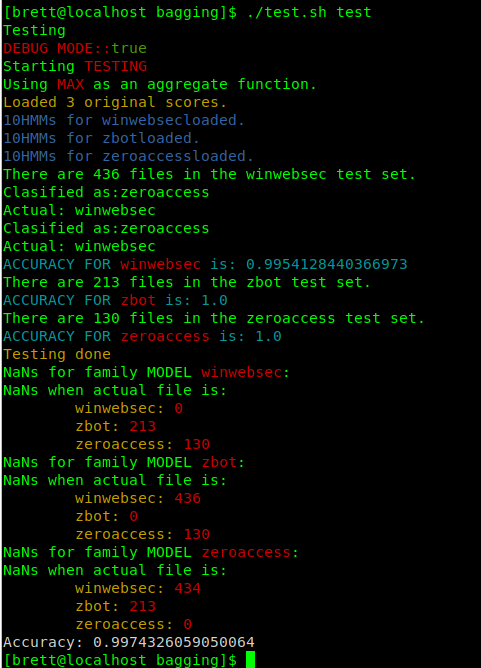
\includegraphics[width=0.5\textwidth]{bagging1.png}
          \caption{Initial results from Bagging.}
          \label{bagging1}
          \end{figure}
 

\end{document}

\iffalse
Todo:
  Sample with replacement for training baggging HMM.

  SVM using the same features as the KNN tests

  DONE Do some ML method (perhaps KNN) where features could be:
  -Entropy
  -Number of distinct opcodes

  Add N-fold validation to bagging
  Trying bagging with replacement
  Use ROC curves

  Add random forrest somewhere?
\fi
